% !TeX root = Protokoll.tex
\subsection{Funktionsweise eines Lasers}
\begin{figure}[b!]
	\centering
	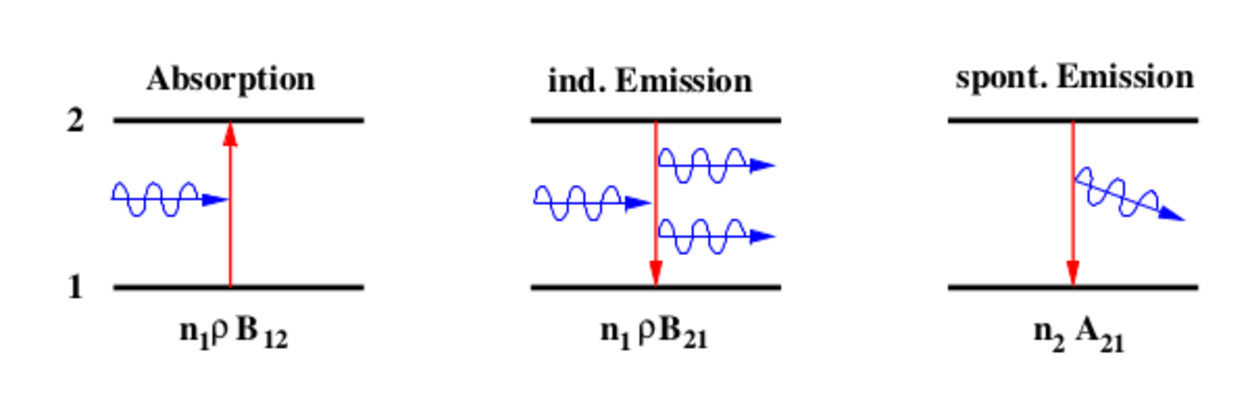
\includegraphics[width = \textwidth]{../Grafiken/Emission.pdf}
	\caption{Hier sind die Emissionen und Absorptionen schematisch dargestellt.\cite{V61}}
\end{figure}
Dieser Abschnitt wurde mithilfe von \cite{V61} erstellt.\\
Grundlegend besteht ein Laser aus drei Komponenten, dem Lasermedium, dem Resonator und einer Pumpquelle.
Die Pumpquelle regt das Lasermedium an, wo durch dies Licht emittiert.
Mithilfe des Resonators wird das Licht öfters durch das Lasermedium geleitet, wodurch mehr Licht emittiert wird das genau die Gleiche Wellenlänge besitzt wie das Licht das es angeregt hat.
Dies hat zur Konsequenz das der Laserstrahl hoher Intensität und  Kohärenz.
Um diesen Prozess genauer zu verstehen, wird das Beispiel eines zwei Niveau Lasers Betrachtet.
Durch ein Photon, das die Energie des Übergangs besitzt, geht das System vom Grundzustand (1) in den angeregten Zustand über.
Die Kohärenz wird dabei durch die Spontane Emission erreicht.
Wenn ein Photon auf das System  trifft, wird ein Photon heraus gelöst, dieses besitzt die selbe Energie, Phase und Ausbreitungsrichtung wie das auslösende Photon.
Dies ist der Effekt der induzierten Emission und der Grund warum Laser so kohärent sind.
Weiter ist es möglich das ein Photon durch spontane Emission emittiert wird, diese Photon besitzt eine Beliebige Phase und Ausbreitungsrichtung.\\
Mithilfe eines Strahlenfeldes $\rho$ lassen sich spontane und induzierte Emission hervorrufen.
Dadurch lässt sich für die Photonenanzahl im System die Gleichungen
\begin{align}
	\dot{N}_A=n_1\rho B_{12}\\
	\dot{N}_{IE}=n_2\rho B_{21}\\
	\dot{N}_{SE}=n_2A_{21}
\end{align}
aufstellen. Hier bezeichnet $n_i$ die Besetzungszahl des Niveaus an, $\dot{N}_A$ ist die Änderung der Photonen durch Absorption, $\dot{N}_{IE}$ die Änderung durch induzierte Emission und $\dot{N}_{SE}$ die Änderung durch spontane Emission.
Weiter sind die Konstanten $A_{21},\ B_{12}$ und $B_{21}$ die Einsteinkoeffizienten und geben die Übergangswahrscheinlichkeiten an.
Es lassen sich daraus nun für den Fall das die Summe der Besetzungszahlen konstant ist die Gleichungen
\begin{align}
	\frac{dn_1}{dt}=&-n_1\rho B_{12}+n_2\rho B_{21}+n_2A_{21}\\
	\frac{dn_2}{dt}=&+n_1\rho B_{12}- n_2\rho B_{21}-n_2A_{21}
\end{align}
aufstellen.
Damit ein Laser dauerhaft Kohärent bleibt, müssen die höheren Niveaus mehr besetzt sein als das Grundniveau, dies wird Besetzungsinversion genannt. 
Das hat zur Folge das spontane Emission seltener auf als die induzierte  Emission.
Um den Zustand der Besetzungsinversion aufrecht zu erhalten, muss dem System dauerhaft Energie hinzugefügt werden.
Dies geschieht zum einem über Die Pumpquelle und zum anderen Durch den Resonator, der das emittierte Licht zurück in das Lasermedium reflektiert, das den Effekt der induzierten Emission hervorruft.
\subsection{Diodenlaser}
\begin{figure}[h!]
	\centering
	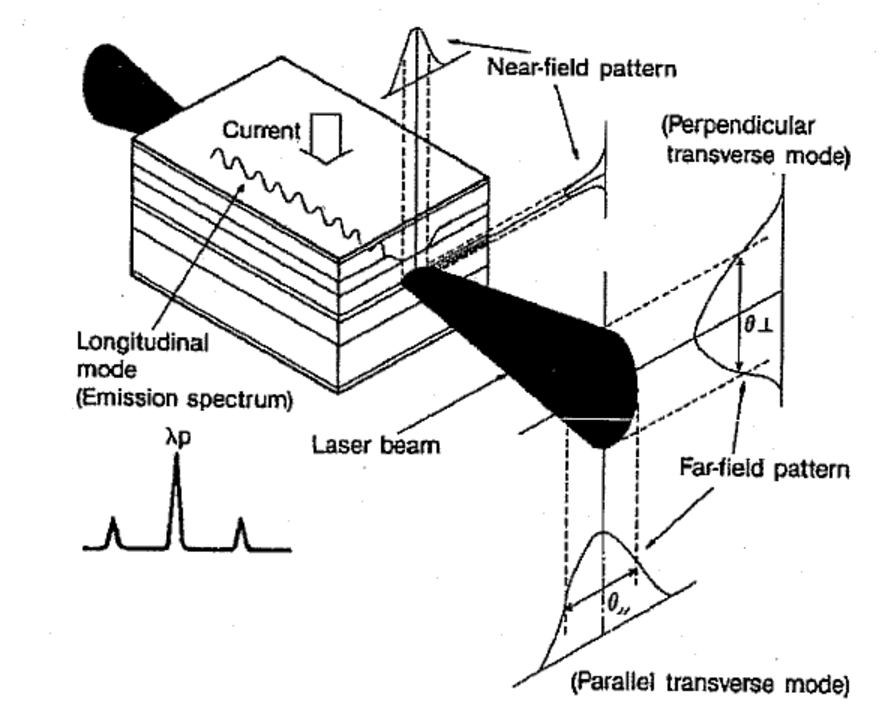
\includegraphics[width = 0.5\textwidth]{../Grafiken/Schematische_Ansicht_Laserdiode.pdf}
	\caption{Skizze des Chips eines Diodenlasers.\cite{V60}\label{fig:Halleiter-Chip}}
\end{figure}
Ein Vorteil des Diodenlasers ist die Bandbreite der Abgedeckten Frequenzen $\Delta \nu = \SI{1}{\mega\hertz}$.
Das Lasermedium wird bei einem Diodenlaser mithilfe eines Halbleiters verwirklicht.
Ein LED-Chip, wie er hier verwendet wird, ist in \cref{fig:Halleiter-Chip} skizziert.
Der Strom fließt von oben nach unten, wodurch Elektronen-Loch-Paare erzeugt werden und bei der Rekombination werden Photonen emittiert.
Damit der Chip kohärentes Licht von sich gibt, muss der Strom einen gewissen Wert übersteigen, darunter funktioniert er wie eine normale LED.
Weiter sind die Brechungsindexes des aktiven Schicht größer als die der benachbarten Schichten, damit wird der Laserstrahl durch die aktive Schicht geführt.
Die beiden Flächen durch die der Strahl führt sind verspiegelt, wobei die eine Seite fast alles Licht reflektiert und die andere Seite teil durchlässig.
Dies Bildet den inneren Resonator (internal Cavity) und gibt dem Laser eine bevorzugte Richtung.
Da der Strahl allerdings sehr divergent ist, wird noch eine Sammellinse eingebaut.
Nach der Sammellinse wird ein Gitter eingebaut.
Dies sorgt dafür das ein groß Teil des gebeugten Lichtes zurück in die Diode strahlt und einen äußeren Resonator bildet (external Cavity).
Der Rest bildet den aus gekoppelten Laserstrahl.
Dieser Aufbau ist in \cref{fig:Aufbau_Gitter_Laserdiode} skizziert.
Ein Nachteil des Diodenlasers ist das er Anfällig für optisches Feedback ist dies wird durch den Aufbau verhindert.
Ebenfalls wird dadurch ermöglicht die Wellenlänge, auf eine bestimmte Wellenlänge festzulegen.
\begin{figure}
	\centering
	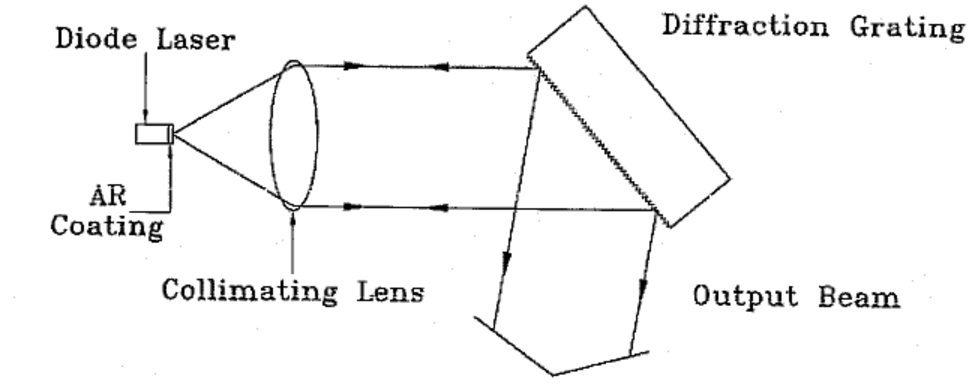
\includegraphics[width = 0.75\textwidth]{../Grafiken/Aufbau_Gitter_Laserdiode.pdf}
	\caption{Hier ist der Aufbau einer Laserdiode mit Gitter skizziert.\cite{V60}\label{fig:Aufbau_Gitter_Laserdiode}}
\end{figure}
\newpage
\subsection{Abstimmen des Lasers}
\begin{figure}[h!]
	\centering
	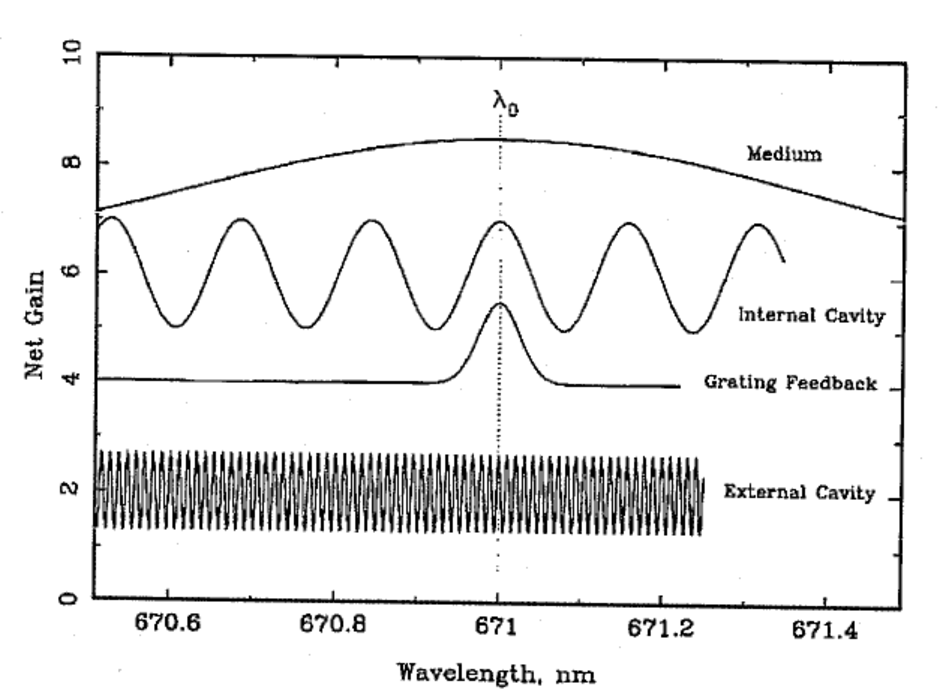
\includegraphics[width = 0.75\textwidth , angle = 1]{../Grafiken/Photon_Gain_Wellenlaenge_Beitraege.pdf}
	\caption{Hier sind die Auswirkungen, der Verschiedenen Effekte auf die Wellenlänge, schematisch dargestellt.\cite{V60}\label{fig:Photon_Gain_Wellenlaenge_Beitraege}}
\end{figure}
Aufgrund der induzierten Emission, emittiert der Laser nur das Licht mit der Wellenlänge, bei der die größte Verstärkung auftritt.
Die Wellenlänge hängt dem nach von verschiedenen Effekten ab.
Diese Werden im folgenden diskutiert und sind in \cref{fig:Photon_Gain_Wellenlaenge_Beitraege} angedeutet.
\subsubsection{Materialabhängigkeit}
Die Wellenlänge des Materials hängt in erster Linie von der Größe der Bandlücke ab.
Dies ist eine Temperaturabhängige Größe, das heißt sie kann durch erhitzen der Diode eingestellt werden.
Da die hervorgerufene Materialverstärkung sehr Breit ist, muss sie nicht genau auf das Maximum der gewünschten Wellenlänge eingestellt werden.
\subsubsection{Innerer Resonator}
Ein Resonator besitzt verschiedene Moden.
Die Moden des inneren Resonators, hängen dabei vom Betriebsstrom der Diode ab.
Zu einem erhitzt der Strom die Diode, was die Wellenlänge beeinflusst, in dem sich der Resonator ausdehnt.
Zum anderen wird die emittierte Wellenlänge erhöht, dadurch das die Trägerkonzentration steigt.
\subsubsection{Das Gitter Feedback}
Das Experiment verwendet die Littrow-Anordnung.
Dabei wird das erste Beugungsmaximum zurück in in den Diodenlaser geleitet.
Wobei die Bragg-Bedingung gilt
\begin{align}
	\lambda = 2d\sin\theta.
\end{align}
Hier ist $d$ der Gitterabstand und $\theta$ der Gitterwinkel.
\subsubsection{Äußerer Resonator}
Die Einflüsse des äußeren Resonators ähneln dem inneren. 
Dadurch das der äußere Resonator so viel größer ist als der innere, liegen die Maxima der longitudinalen Moden enger zusammen.
Durch ändern der Position des Gitters ändert sich die Länge des äußeren Resonators und somit die Form der Moden.
\subsection{Modensprünge}
\begin{figure}[h!]
	\centering
	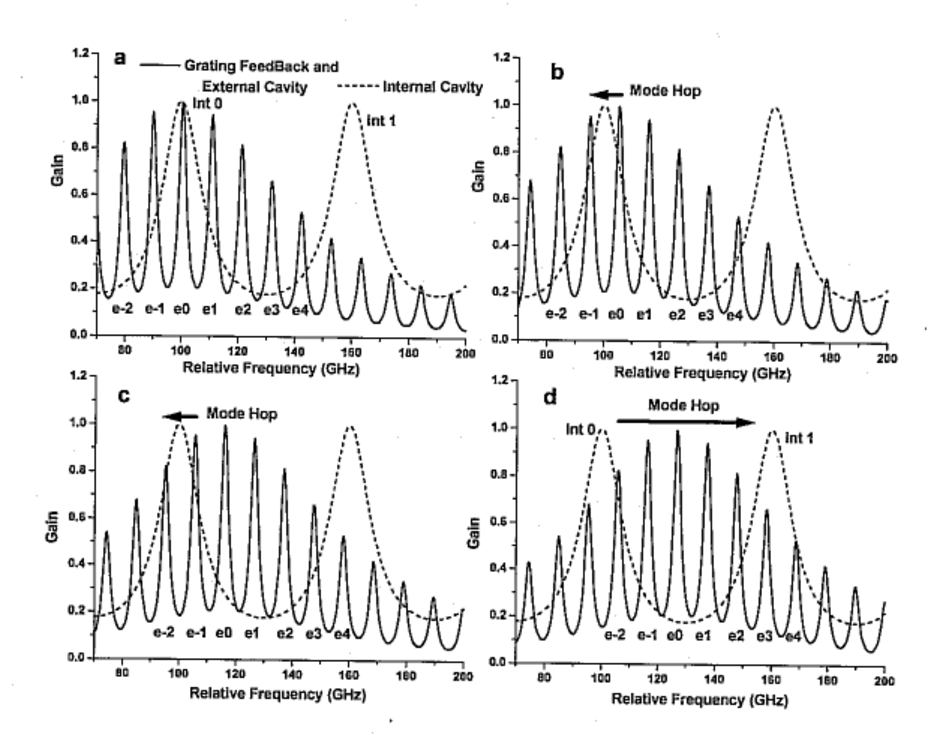
\includegraphics[width = 0.75\textwidth, angle = 1]{../Grafiken/Moden_Spruenge.pdf}
	\caption{Hier ist die Kombination des Gitter Feedback und des Äußeren Resonators sowie extra der innere Resonator Dargestellt, für Verschiedene Winkel.\cite{V60}\label{fig:Moden_Spruenge}}
\end{figure}
In \cref{fig:Moden_Spruenge} ist eine Kombination des äußeren Resonator und des Gitter Feedbacks sowie der innere Resonator eingezeichnet.
Von Bild a bis zu Bild d wird der Gitterwinkel immer weiter Verringert.
In Bild a ist der Winkel so eingestellt, dass das Maximum e0 der Äußeren Einflüsse auf dem Maximum Int0 des inneren Resonators liegt.
